\documentclass{article}

\usepackage[normalem]{ulem}
\usepackage{fancyhdr}
\usepackage{graphicx}
\pagestyle{fancyplain}

\title{Momentum and Newton's laws}
\author{Todd Davies}
\date{\today}

\begin{document}

\rhead{Momentum and Newton's laws}
\lhead{\today}

\maketitle

\section*{Newton's three laws}
\thispagestyle{empty}
\label{sec:NewtonSThreeLaws}
Learn these, sometimes you've got to state them on the exam.
\subsection*{Newton's first law}
\textbf{Definition:} \textit{An object will remain at rest or keep travelling at a constant velocity unless it is acted on by an external force.}\\
Another way of saying this is that the momentum of an object is constant unless an external force acts upon it.
\subsection*{Newton's second law}
\textbf{Definition:} \textit{The net force acting on an object is directly proportional to the rate of change of the linear momentum of that object. The net force and the change in momentum are in the same direction.}\\
This means that 
\[
	net\:force \propto rate\:of\:change\:of\:momentum
\]
Which can also be written as:
\[
	F = \frac{\Delta p}{\Delta t}
\]
\textit{N.b. the Newton is defined so that there doesn't need to be a constant to turn the proportional sign into an equals sign.}\\
Where:
\begin{center}
	\begin{tabular}{|l|l|l|}
		\hline
			Quantity & Abbreviation & Unit \\ \hline
			Change in momentum & $\Delta p$ & Kilogram meter per second ($kgms^{-1}$) \\ \hline
			Change in time & $\Delta t$ & Second ($s$) \\ \hline
			Force & $F$ & Newton ($N$) \\ \hline
	\end{tabular}
\end{center}
This can also be defined as:\\
\textbf{Alternate definition:} \textit{The net force on an object is equal to the rate of change of it's momentum. The next force and the change in momentum are in the same direction}
\subsubsection*{An extension of the second law}
We can change $\Delta p$ into $mv - mu$. Since $m$ is constant, we can take it out as a factor like so:
\[
	F = m\frac{v - m}{\Delta t}
\]
You may have noticed that we can then substitute the second half of the equation for acceleration (since acceleration is the rate of change of the speed):
\[
	F = ma
\]
\subsection*{Newton's third law}
This is the easy one! It's definition is as follows: \textit{When two bodies interact, the forces that they exert on each other are equal and opposite}.\\
These two forces are always:\\
However, most people know it by this definition:
\textbf{Alternate definition:} \textit{Every action has an equal and opposite reaction.}

\begin{itemize}
	\item Of the same type (e.g. magnetic)
	\item Are equal in magnitude
	\item Are opposite in direction
	\item Act on different bodies (usually the two bodies that are creating the force)
\end{itemize}

\section*{Impulse}
Impulse is defined as the \textit{rate of change of momentum} or $Impulse = F \times t$. The unit of impulse is the \textit{Newton second ($Ns$)}.\\
You can find the impulse by working out the area of a force time graph (useful if the force isn't constant). Here's a force time graph with the area highlighted:
\begin{figure}[htbp]
	\centering
		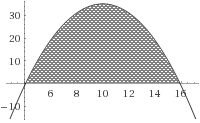
\includegraphics{graph.png}
	\caption{The area under a Force Time graph is the impulse}
\end{figure}


\section*{Derivation of the law of conservation of momentum from Newton's second and third laws}
If we imagine two trolleys colliding. Both have the same speed and mass but are moving towards each other in opposite directions. 
\begin{itemize}
	\item The total momentum is therefore zero.
	\item When they collide, they decelerate at the same rate (but in opposite directions) and so there is two forces that are equal and opposite.
	\item The time of the collision is the same for each trolley, so the impulse for each trolley ($F \Delta t$) is equal in magnitude, but acts in opposite directions.
	\item The impulse in each trolley is the same as it's change in momentum.
\end{itemize}

We can conclude that if one trolley gains momentum in one direction, then the other gains an equal amount in an opposite direction and the total momentum in the system is the same.

\section*{Questions to practice}
\textbf{Question 1}\\
A 1000kg spaceship is stationary in space. It's engines are activated for two minutes and provide a continuous force of 20N for this time, after which they deactivate.

\begin{enumerate}
	\item First, find the velocity of the spaceship after it's engines have stopped.
	\item Now calculate the acceleration of the spaceship and work done by the engines.
	
\end{enumerate}

\noindent
\textbf{Answers}
\begin{enumerate}
	\item \[
		F = \frac{\Delta p}{t}
		\]
		So we can use this to find the momentum, and sub in $\Delta p = mv - mu$ to find the velocity.
		\[
			20 = \frac{1000v - 0}{120}
		\]
		\[
			\frac{20 \times 120}{1000} = v
		\]
		\[
			v = \uline{2.4ms^{-1}}
		\]
	\item Finding the acceleration is easy, just use $F = ma$:
	\[
		20 = 1000a
	\]
	\[
		a = \uline{0.020ms^{-2}}
	\]
	The work done is equal to the change in kinetic energy. Since the kinetic energy was zero to begin with, we just need to find the final kinetic energy of the spaceship:
	\[
		KE = \frac{1}{2}mv^2
	\]
	\[
		KE = \frac{1}{2} \times 1000 \times 2.4^2
	\]
	\[
		KE = \uline{2880 Joules}
	\]
\end{enumerate}


\end{document}
